\chapter{組版システムReVIEWでQiitaから同人誌原稿を作る}
\label{chap:qiita2review}
 \begin{center} 
河野悦昌  \textbf{秘密結社オープンフォース 送信}

 \end{center} 
\section{markdownからReVIEW}
\label{sec:5-1}

ReVIEW+markdown で数式の入った薄い本を書く
http://qiita.com/nanbuwks/items/9b00e8012e328de6e440
というのを書きました。

何人かでこういうのやるときに、オンライン投稿するやりかたを考えます。

\section{Qiitaで書くメリット}
\label{sec:5-2}

Qiita ってよくできていて、割とラフな操作でもいい感じに作ってくれます。

\begin{itemize}
\item オンラインで投稿、書いてる途中でリアルタイムにレンダリング結果を確認
\item 画像ドラッグ\&ドロップで投稿できる
\item URLとか自動でリンクに変換してくれる
\end{itemize}

これを使うやり方を考えてみました。

\section{catalog.yml}
\label{sec:5-3}

章立てはこうなってます

\begin{reviewemlist}
PREDEF:

CHAPS:
  {-} 1.re

APPENDIX:

POSTDEF:
\end{reviewemlist}

ここの、CHAPSに複数人の原稿を登録するという感じです。

\section{ひとつの記事を元に原稿を作ってみる}
\label{sec:5-4}

Pi board (Single Board Computer) and Allwinner
http://qiita.com/nanbuwks/items/7f5fd126b8581e6d1a74

を元にしてみます。

まず、

\begin{reviewemlist}
review{-}init piallwinner
cd piallwinner
\end{reviewemlist}

catalog.ymlと config.yml を編集しておきます。

図をダウンロードします

\begin{reviewemlist}
cd images
wget http://qiita.com/nanbuwks/items/7f5fd126b8581e6d1a74 {-}k {-}H {-}r {-}l 1 {-}nH {-}nd {-}A png,PNG,jpg,JPG,jpeg,JPEG,html  {-}R txt
cd ..
\end{reviewemlist}

markdownファイルをダウンロードします。

\begin{reviewemlist}
wget http://qiita.com/nanbuwks/items/7f5fd126b8581e6d1a74.md
\end{reviewemlist}

imgファイルをローカルに変換します。

\begin{reviewemlist}
ruby qiitamd.rb 7f5fd126b8581e6d1a74.md \textgreater{} 1.md
md2review 1.md \textgreater{} 1.re
rake pdf
\end{reviewemlist}

変換するスクリプト qiitamd.rb です

\begin{reviewemlist}
\#\#!/usr/bin/env ruby

while line = gets
  line.chomp!
  if md1 = line.match(/(\textasciicircum{}!\reviewbackslash{}[.*?\reviewbackslash{}]\reviewbackslash{}()/)
    if md2 = line.match(/([\textasciicircum{}\reviewbackslash{}/]*\reviewbackslash{}))/)
\#\#      puts line
\#\#      print md1[0],"\reviewbackslash{}n"
\#\#      print md1[1],"\reviewbackslash{}n"
\#\#      print md2[0],"\reviewbackslash{}n"
\#\#      print md2[1],"\reviewbackslash{}n"
\#\#      print "\reviewbackslash{}n"
\#\#      print md2[0],md1[0],"\{\reviewbackslash{}n"
      print md1[0]
      print "images/"
      print md2[1]
      print "\reviewbackslash{}n"
    else
      puts line
    end
  else
   puts line
  end
end

\end{reviewemlist}

\section{複数の記事を元に原稿を作ってみる}
\label{sec:5-5}

\begin{reviewemlist}
PREDEF:

CHAPS:
  {-} 1.re
  {-} 2.re
  {-} 3.re

APPENDIX:

POSTDEF:
\end{reviewemlist}

として、2.re や 3.re に上のような原稿を当てはめるといいでしょう。

\section{画像を縮小する}
\label{sec:5-6}

Qiitaは画像をアップロードすると、はみ出る画像は横幅100\%でビューするように画面を作ってくれます。紙媒体の場合は多くは100\%だと良くないですね。50\%ぐらいの大きさを使うようにするには?

通常の画像をアップロードすると以下のようなmarkdownとなります。
@\textless{}tt\textgreater{}\{
![ファイル名](images/c19f0873{-}8b39{-}9405{-}1486{-}8cfd43e38d78.jpeg)
\}

\begin{reviewimage}
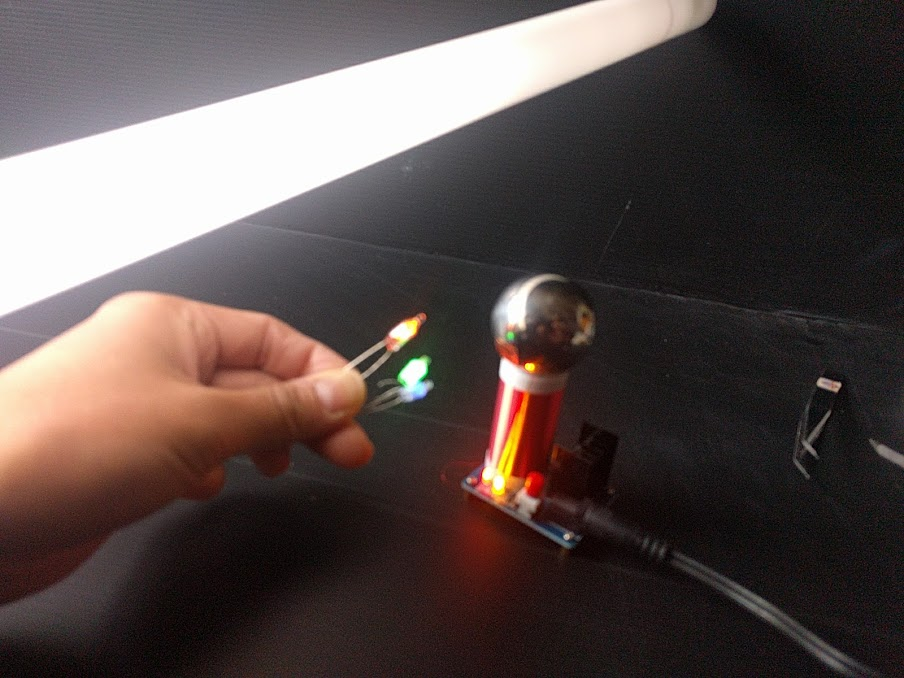
\includegraphics[width=\maxwidth]{./images/c19f0873-8b39-9405-1486-8cfd43e38d78.jpeg}
\caption{ファイル名}
\label{image:qiita2review:c19f0873-8b39-9405-1486-8cfd43e38d78}
\end{reviewimage}

Qiitaでは、imgタグに書き換えると小さくなります。
@\textless{}tt\textgreater{}\{
\textless{}img width="50\%" alt="ファイル名" src="https://qiita{-}image{-}store.s3.amazonaws.com/0/139524/c19f0873{-}8b39{-}9405{-}1486{-}8cfd43e38d78.jpeg"\textgreater{}
\}

\textless{}img width="50\%" alt="ファイル名" src="https://qiita{-}image{-}store.s3.amazonaws.com/0/139524/c19f0873{-}8b39{-}9405{-}1486{-}8cfd43e38d78.jpeg"\textgreater{}

この解決方法は、GitHubなどでも同様です。
タグをいちいち書き換えないといけないのでメンドクサイですね。
markdownの拡張でできないかと思ったのですがそういうのは無さそうです。

仕方がないので、Qiita上では100\%で表示されるけれども、PDFに変換した時に任意の大きさになるようにする。

「画像を初期化するスクリプト」
http://qiita.com/nanbuwks/items/9b00e8012e328de6e440\#\%E7\%94\%BB\%E5\%83\%8F\%E3\%82\%92\%E7\%B8\%AE\%E5\%B0\%8F\%E3\%81\%99\%E3\%82\%8B\%E3\%82\%B9\%E3\%82\%AF\%E3\%83\%AA\%E3\%83\%97\%E3\%83\%88

を使うと、

\begin{reviewimage}
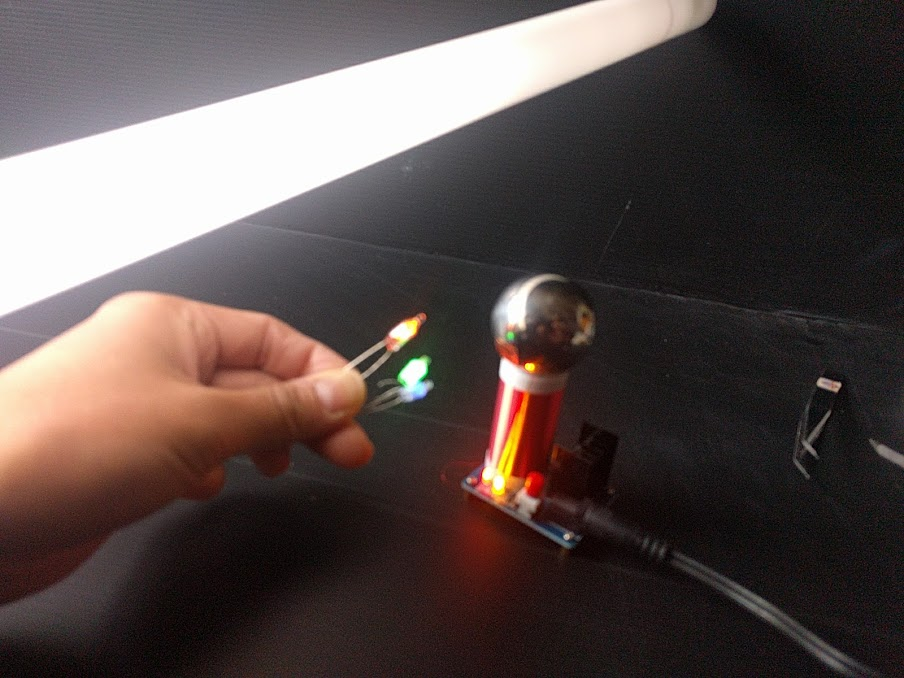
\includegraphics[width=0.5\maxwidth]{./images/c19f0873-8b39-9405-1486-8cfd43e38d78.jpeg}
\caption{ファイル名}
\label{image:qiita2review:c19f0873-8b39-9405-1486-8cfd43e38d78}
\end{reviewimage}

\begin{reviewemlist}
[scale=0.5]![ファイル名](https://qiita{-}image{-}store.s3.amazonaws.com/0/139524/c19f0873{-}8b39{-}9405{-}1486{-}8cfd43e38d78.jpeg)
\end{reviewemlist}

と書けば、Qiita上では大きく、紙媒体に印刷したときには50\%で印刷される。
けれども
[scale=0.5]というのが表示されてしまう。

少し書式を変更。

\begin{reviewemlist}
[]( scale=0.5 )![ファイル名]( https://qiita{-}image{-}store.s3.amazonaws.com/0/139524/c19f0873{-}8b39{-}9405{-}1486{-}8cfd43e38d78.jpeg )
\end{reviewemlist}

とした。

\begin{reviewimage}
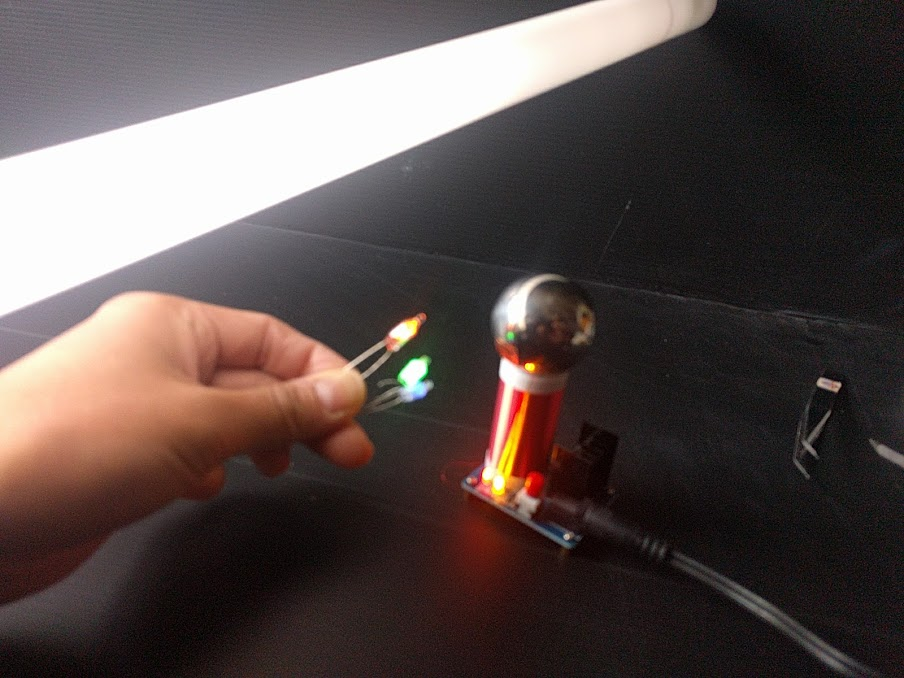
\includegraphics[scale=0.5 ]{./images/c19f0873-8b39-9405-1486-8cfd43e38d78.jpeg}
\caption{ファイル名}
\label{image:qiita2review:c19f0873-8b39-9405-1486-8cfd43e38d78}
\end{reviewimage}

しかしながら md2review でエラーが起こる

\begin{reviewemlist}
 md2review qiita2review2.md
/var/lib/gems/2.3.0/gems/md2review{-}1.11.0/lib/redcarpet/render/review.rb:299:in `remove\textunderscore{}inline\textunderscore{}markups': undefined method `gsub' for nil:NilClass (NoMethodError)
    from /var/lib/gems/2.3.0/gems/md2review{-}1.11.0/lib/redcarpet/render/review.rb:191:in `link'
    from /var/lib/gems/2.3.0/gems/md2review{-}1.11.0/lib/md2review/markdown.rb:13:in `render'
    from /var/lib/gems/2.3.0/gems/md2review{-}1.11.0/lib/md2review/markdown.rb:13:in `render'
    from /var/lib/gems/2.3.0/gems/md2review{-}1.11.0/bin/md2review:54:in `\textless{}top (required)\textgreater{}'
    from /usr/local/bin/md2review:22:in `load'
    from /usr/local/bin/md2review:22:in `\textless{}main\textgreater{}'

\end{reviewemlist}

\begin{reviewemlist}

[]( scale=0.5 )

\end{reviewemlist}

という書き方はmarkdownのコメントアウトなので、これでエラーが起こるとは情けないぞ。

\begin{reviewemlist}
[](
)
\end{reviewemlist}

こんなのでも同様のエラー。
仕方がないので通常のコメントはふつーに消去、\texttt{scale=0.5 )} は \texttt{[scale=0.5]} にするフィルタを作り、md2reviewをかける前に適用するようにしよう。

「preprosess.rb」

\begin{reviewemlist}
\#\#!/usr/bin/env ruby
\#\# this is not support \textdollar{}...\textdollar{} in inline htmltag,link,image.
codeBlock=false
incomment=true
while line = gets
  line.chomp!
  if ( codeBlock == false \&\& md1 = line.match(/\textasciicircum{}```/))
      codeBlock=true
      puts line
  elsif ( codeBlock == true \&\& md1 = line.match(/\textasciicircum{}```/))
      codeBlock=false
      puts line
  elsif ( codeBlock == false \&\& md1 = line.match(/\textasciicircum{}\reviewbackslash{}[\reviewbackslash{}]\reviewbackslash{}(\reviewbackslash{} *(scale=.*)\reviewbackslash{} *\reviewbackslash{})!\reviewbackslash{}[.*\reviewbackslash{}]\reviewbackslash{}(.*\reviewbackslash{})/))
      md2 = line.match(/\textasciicircum{}\reviewbackslash{}[\reviewbackslash{}]\reviewbackslash{}(\reviewbackslash{} *scale=.*\reviewbackslash{} *\reviewbackslash{})(!\reviewbackslash{}[.*\reviewbackslash{}]\reviewbackslash{}(.*\reviewbackslash{}))/)
      print "[" + md1[1] + "]" + md2[1]
  elsif ( codeBlock == false )
    offset=0
    while md1 = line.index("[](",offset) do
      thereistex=false
      if ( md2 = line.match(/\reviewbackslash{}\textdollar{}.*?\reviewbackslash{}\textdollar{}/))
        thereistex=true
      end
      inlinecode="nocode"
      inlinetex="notex"
      for  num in offset..md1{-}1
         ch = line[num]
         if ( ch == "`" \&\& inlinecode=="nocode" )
             inlinecode="starting"
         elsif ( ch != "`" \&\& inlinecode=="starting" )
            inlinecode="incode"
         elsif ( ch == "`" \&\& inlinecode=="incode" )
            inlinecode="ending"
         elsif ( ch != "`" \&\& inlinecode=="ending" )
            inlinecode="nocode"
         elsif ( ch == "\textdollar{}" \&\& inlinecode=="nocode" \&\& inlinetex=="notex" \&\& thereistex==true )
            inlinetex="intex"
         elsif ( ch == "\textdollar{}" \&\& inlinecode=="nocode" \&\& inlinetex=="intex" )
            inlinetex="notex"
         end
         print ch
      end
      offset=md1+4
      num=offset{-}1
      if ( inlinetex!="notex" \textbar{}\textbar{} inlinecode!="nocode")
      else
        incomment=true
        while incomment==true do
          if ( line.length \textless{} num )
            if ( line=gets )
              num=0
            else
              incomment=false
            end
          end
          ch=line[num]

          if ( ch == ")" )
            incomment=false
          end
          num=num+1
          offset=num
        end
      end
    end
    line=line[offset,line.length]
    puts line
  else
    puts line
  end
end

\end{reviewemlist}

制限

汚いコードになってしまったし、
